\documentclass[11pt, a4paper]{report}
%--------------Importación de paquetes (preámbulo)--------------%
%--------------Elección del idioma español--------------%
\usepackage[spanish,es-noshorthands, es-tabla]{babel}
%--------------------------------------------------------------%
%-Elección de codificación y caracteres especiales-%
\usepackage[utf8]{inputenc}
\usepackage[T1]{fontenc}
% \usepackage{anyfontsize}
% \usepackage{t1enc}
%--------------------------------------
\usepackage{lmodern}
%Caracteristicas matematicas: simbolos, caracteres, etc%
% \usepackage{amsmath,amsfonts,amssymb,amsthm}
% \usepackage{indentfirst}
% \usepackage{anysize}

%-----Caracteristicas para el manejo de graficos-----%
%\usepackage{graphics}%
\usepackage{graphicx}
% \usepackage{transparent}
% \usepackage{eso-pic}
%\usepackage[lofdepth,lotdepth]{subfig}
\usepackage{float}
\usepackage{pgf,tikz,pgfplots,mathrsfs}
% \usepackage{pstricks-add}
% \usetikzlibrary{calc}
% \usetikzlibrary{babel}
% \usepackage{tikzpagenodes}
\usepackage{lipsum}
\usepackage[font=small,labelfont=bf]{caption}
%\usetikzlibrary{arrows,patterns}
\pgfplotsset{compat=1.15}

% \usepackage{pst-node}
% \usepackage{pst-plot}
% \usepackage{psfrag}
%__Manejo de múltiples columnas
\usepackage{multicol}
%__Manejo de entrelineado
% \usepackage{setspace}
%__Manejo de color
% \usepackage{color}
% \usepackage{xcolor}
%__Manejo de tablas
% \usepackage{colortbl}
% \usepackage{rotating}
\usepackage{multirow}
% \usepackage{booktabs}
% \usepackage{tabularx}
\usepackage{tabulary}
% \usepackage{bigstrut}
\usepackage{longtable,lscape}
% \usepackage{array}
%__Manejo de índice
% \usepackage{makeidx}
%__Manejo de cabecera y pies de pagina
\usepackage{fancyhdr}
%__Manejo de la enumeración
% \usepackage{enumitem}

%---------------Otros paquetes---------------%
% \usepackage{pdflscape}
% \usepackage{subfigure}
% \usepackage{enumerate}
% \usepackage{textcomp}
% \usepackage{afterpage}
\usepackage{background}
%------------ Paquetes Para codigo-----------%
% \usepackage{verbatim}
% \usepackage{moreverb}
% \usepackage{fancybox}
\usepackage{pythontex}
%--------------------------------------------------------------%
%Autor%
\author{CISMID\\Kevin Steve Huerta Gonzales}
%%%%%%%  Comandos Personalizados %%%%%%
\newcommand{\multlinecomment}[1]{\directlua{-- #1}}
%%%%%%---%%% algunas configuraciones por implementar
\captionsetup{%
  font={small}, % small font size
  labelfont={bf,sf},      % label in bold, sans-serif
  singlelinecheck=true, % centered single-lined captions
  format=hang,             % indention=1cm ---> plain
  labelsep={colon},         % default separator: none, colon, period, space, quad, newline, endash
}
\usepackage[
            pdftex,
            pdfauthor={Joseph Jaramillo},
            pdftitle={Informe reporte sísmico},
            pdfsubject={UTN},
            pdfkeywords={Computer UNIVAC Evolutionary},
            pdfproducer={TeXLive},
            pdfcreator={pdflatex, or other tool},
            colorlinks=true,
            linkcolor=black]{hyperref}
%---------------------------------------------------------------%
\graphicspath{ {Figures/} }
\setlength{\parindent}{0em}
\topmargin=0.5cm
\usepackage[lmargin=2cm,rmargin=2cm,bottom=1cm]{geometry}
%%%%%% --- generando caja de pagina como background
\DefineNamedColor{named}{Cyan}{cmyk}{250,250,250,250}
\backgroundsetup{
scale=1,
angle=0,
color=Cyan,
opacity=0.15,
contents={ %\transparent{0.4}

\includegraphics[width=100mm]{Logos/logo_cismid.png}
}
}

%---------------------------------------------------------------%
\title{CENTRO DE MONITOREO SÍSMICO DEL CISMID-FIC-UNI \\
RED NACIONAL DE ACELERÓGRAFOS (REDACIS)\\
INFORME PRELIMINAR\\
}

%%  -------Encabezado -------%%%
\lhead{\vspace{-1cm} \begin{picture}(0,0) \put(0,0){
\includegraphics[width=18mm]{Logos/logo_uni}} \end{picture}}
\rhead{\vspace{-1cm} \begin{picture}(0,0) \put(-70,0){
\includegraphics[width=27mm]{Logos/logo_cismid}} \end{picture}}
\chead{\vspace{-0.5cm} UNIVERSIDAD NACIONAL DE INGENIERÍA\\
FACULTAD DE INGENIERÍA CIVIL\\
CENTRO PERUANO JAPONÉS DE INVESTIGACIONES\\
SÍSMICAS Y MITIGACIÓN DE DESASTRES\\
\vspace{-0.5cm} }


\renewcommand{\headrulewidth}{1pt}
\renewcommand{\headrule}{\hbox to\headwidth{\color{Cyan}\leaders\hrule height \headrulewidth\hfill}}
\renewcommand{\footrulewidth}{1pt}
\renewcommand{\footrule}{{\color{Cyan}\vskip-\footruleskip\vskip-\footrulewidth \hrule width\headwidth height\footrulewidth\vskip\footruleskip}}
%\futurelet\TMPfootrule\def\footrule{{\color{blue}\TMPfootrule}}
\setlength\headheight{40.0pt}
\addtolength{\textheight}{-100.0pt}
\cfoot{\scriptsize AV. TÚPAC AMARU N° 1150 – LIMA 25 – PERÚ – Apartado Postal 31-250 Lima 31\\
		Teléfono (511)482-0777, (511)482-0804, (511)482-0790   Fax: (511)481-0170 \\
		e-mail: director@uni.edu.pe   http://www.cismid.uni.edu.pe
		}
\pagestyle{fancy}

%%%%%
%-------------------CUERPO-------------------%
\begin{document}

% \listoffigures

% \listoftables

% \newpage


\begin{pycode}
from Python_tools.core import Event
import pandas as pd

event = Event.load_event_properties('D:/SHM/code-jj/Report/Event.sav')

lugar = event.epicenter["Place"].iloc[0]
fecha = event.epicenter["Date"].iloc[0]
hora_local = event.epicenter["Local Hour"].iloc[0]
hora_UTC = event.epicenter["UTC Hour"].iloc[0]
referencia = event.epicenter["Venue"].iloc[0]
institucion = event.epicenter["Institution"].iloc[0]
latitud = event.epicenter["Latitude"].iloc[0]
longitud = event.epicenter["Longitude"].iloc[0]
profundidad =  event.epicenter["Depth"].iloc[0]
magnitud = event.epicenter["Magnitude"].iloc[0]
nstations = str(len(event.station)).zfill(2)

\end{pycode}

\begin{center}
\centering 
\textbf{CENTRO DE MONITOREO SÍSMICO DEL CISMID-FIC-UNI \\
RED DE MONITOREO DE EDIFICACIONES\\}
\vspace{0.3cm}

\textbf{INFORME PRELIMINAR\\}
\vspace{0.3cm}

\textbf{Acelerogramas del Sismo de \py{lugar} del \py{fecha}}
\vspace{0.25cm}
\end{center}

El \py{fecha} a las \py{hora_local} (hora local), ocurrió un sismo con epicentro a \py{referencia} (Fuente: \py{institucion}). Las características sísmicas del evento 
se resumen en la \textbf{Tabla (\ref{tab:tab01})} y la ubicación del epicentro, así como de las estaciones 
acelerográficas más cercanas, se muestra en la \textbf{Figura (\ref{tab:tab01})}. \\

\begin{figure}[H]
    \begin{multicols}{2}
        \begin{minipage}[c]{7.5cm}
            \centering
            \renewcommand{\arraystretch}{1.8}
            \captionof{table}{Datos sísmicos (Fuente: \py{institucion})} \label{tab:tab01}
            \begin{tabulary}{7.0cm}{|l|C|}
                
            \hline
            Hora local (UTC-5): & \py{hora_local} \\ \hline
            Hora UTC 0: & \py{hora_UTC} \\ \hline
            Latitud ($^{\circ}$): & \py{latitud} \\ \hline
            Longitud ($^{\circ}$): & \py{longitud} \\ \hline
            Profundidad (km): & \py{profundidad} \\ \hline
            Magnitud (ML): & \py{magnitud} \\ \hline
            Lugar de referencia: & \py{referencia}. \\ 
            \hline
            \end{tabulary}
        \end{minipage}
    
        \hspace{0.5cm}
    
        \begin{minipage}[c]{8.2cm}
            \centering %%\captionsetup{format = hang, width=8cm}
            \setlength\fboxsep{0pt}
            \setlength\fboxrule{0.3pt}
            \captionof{figure}{Epicentro y estaciones cercanas.}  \label{fig:fig01}
            % \begin{figure}
                \fbox{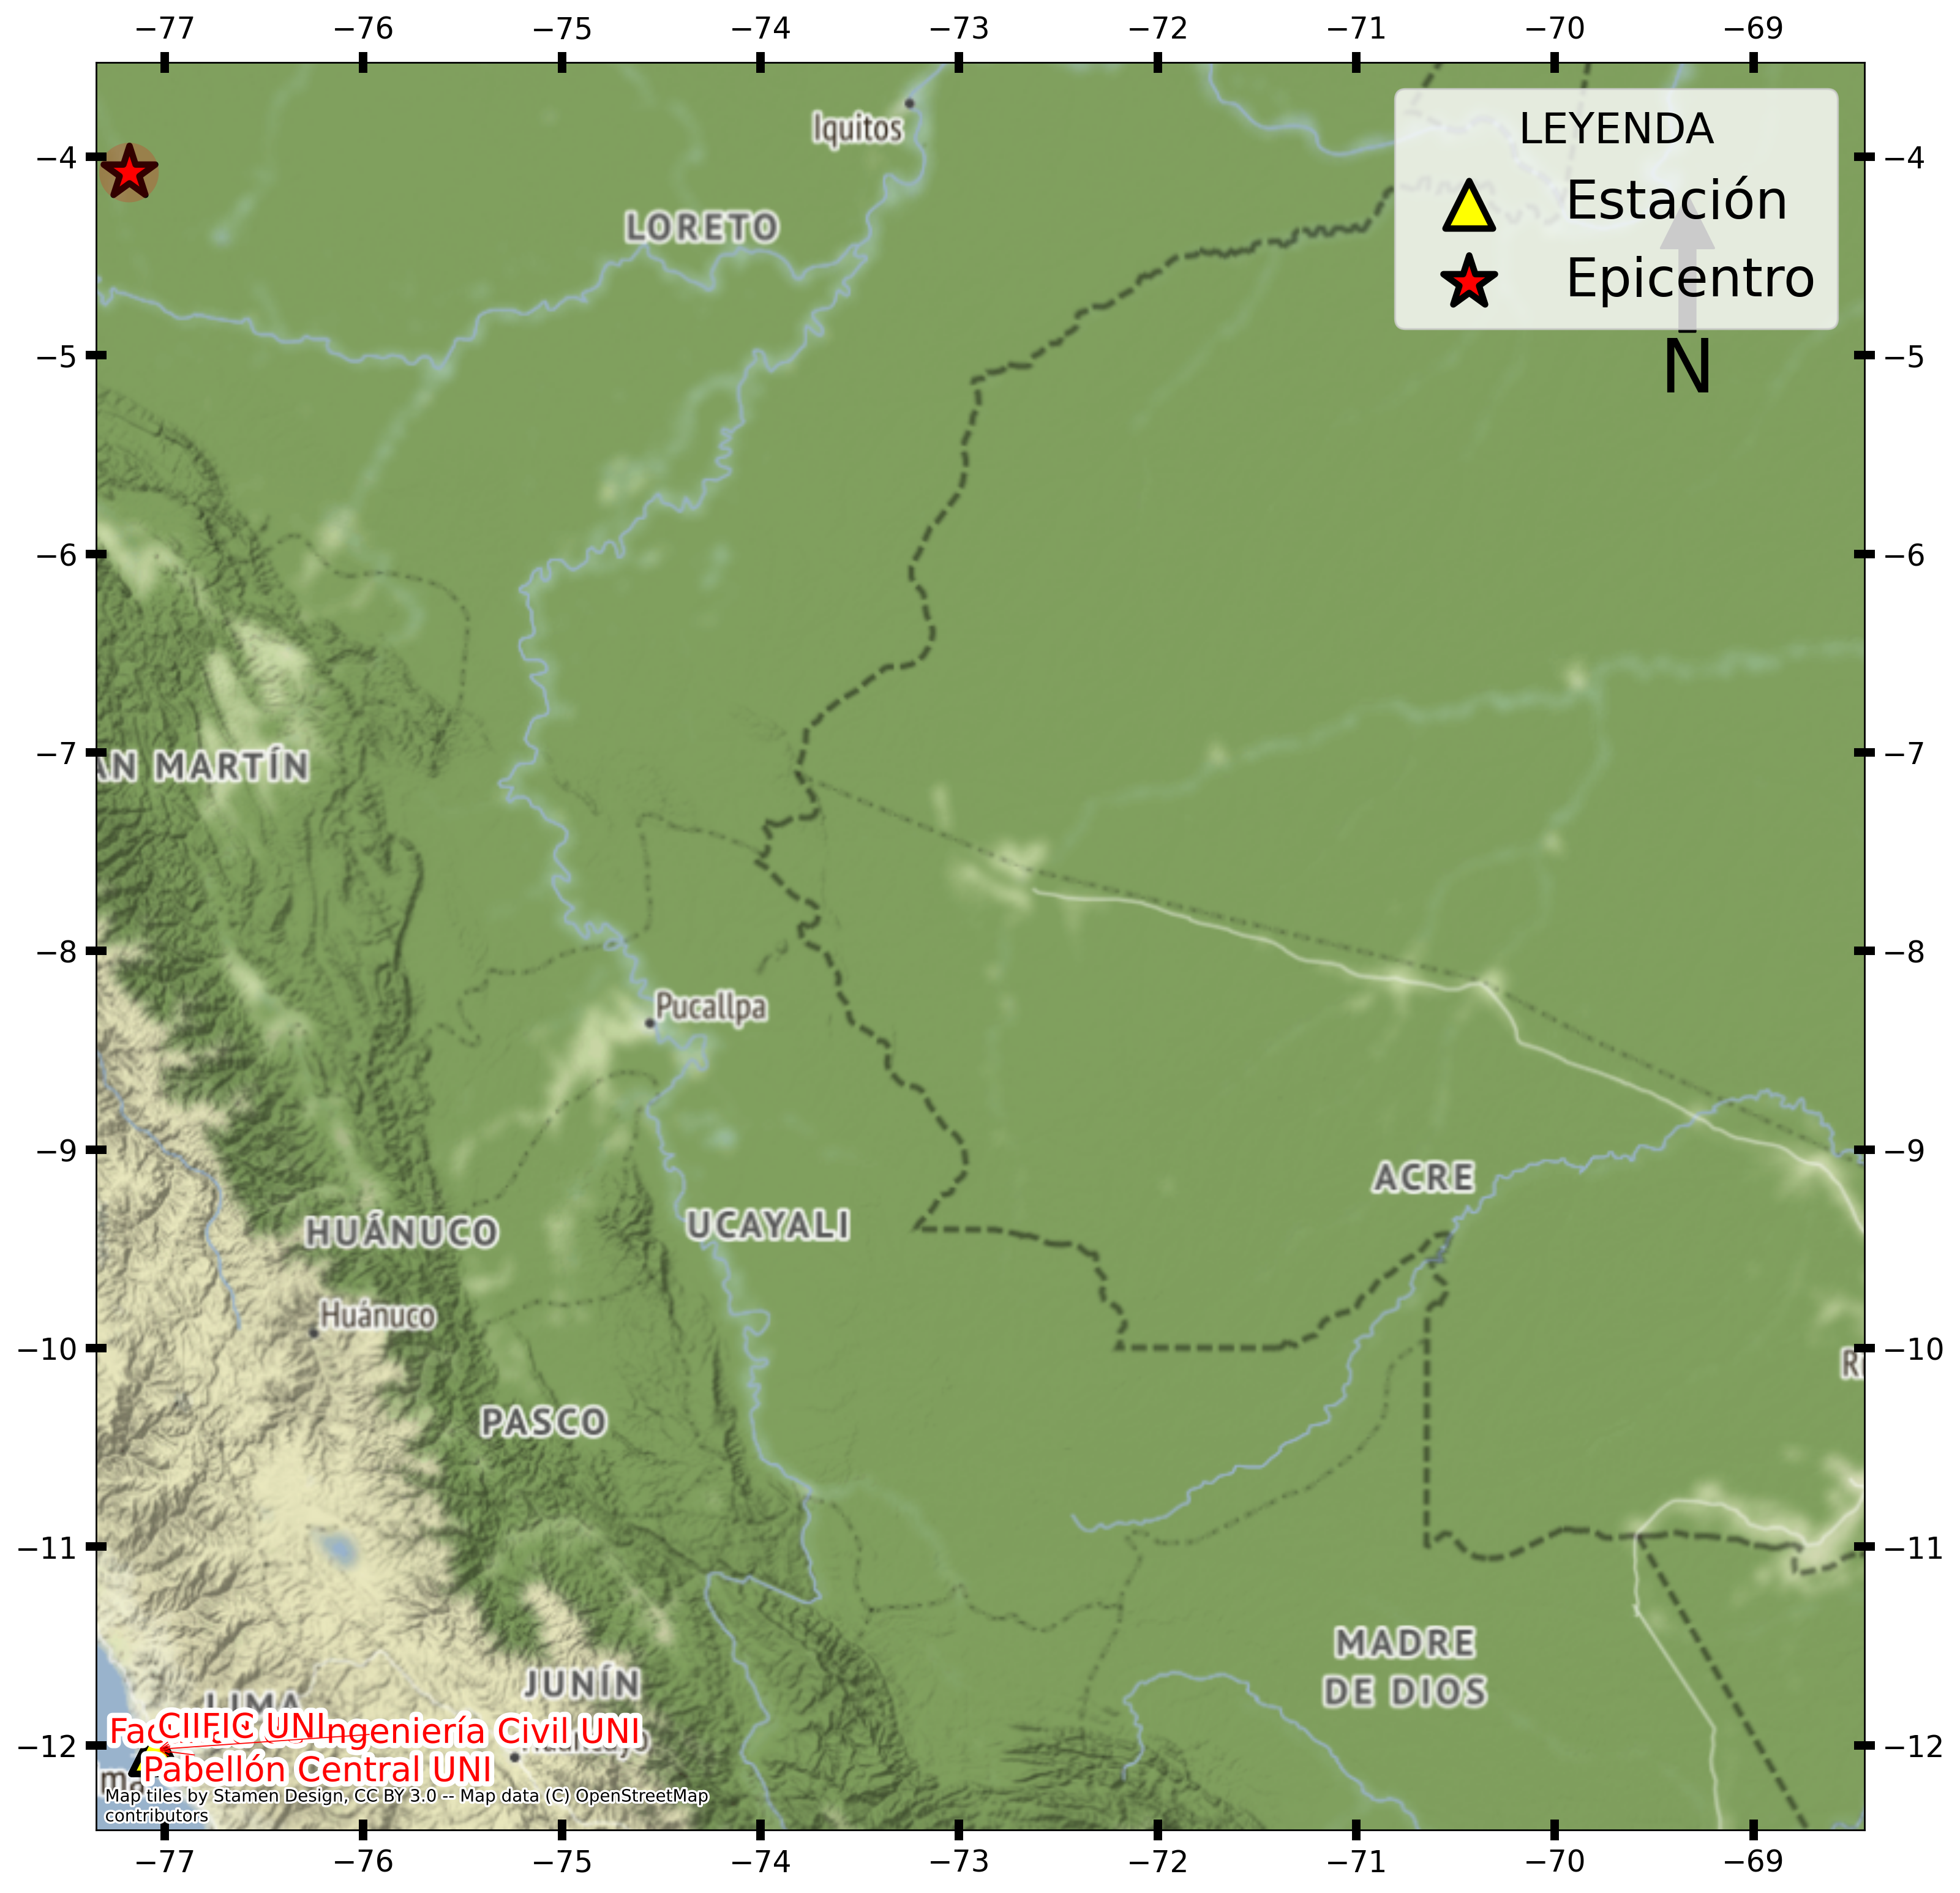
\includegraphics[trim={1mm 0.5mm 1mm 0.5mm},clip,width=1.0\textwidth]{Mapa01.png}}
            % \end{figure}
        \end{minipage}
    \end{multicols} 
\end{figure}

\vspace{1cm}

\noindent
En este reporte, la Red de Monitoreo de Edificaciones (REMOED) del Centro Peruano Japonés de Investigaciones Sísmicas y Mitigación
de Desastres (CISMID) FIC-UNI presenta de manera preliminar, los registros sísmicos obtenidos de este evento correspondiente a 
\py{nstations} estaciones acelerográficas ubicadas en la ciudad de Lima, cuyos valores de aceleración máxima, para cada 
componente, y localizaciónes se muestran en la \textbf{Tabla (\ref{tab:tab02})} y \textbf{Figura (\ref{fig:fig02})} respectivamente.\\

\begin{pycode}
pga_max = round(event.max_station["Max_pga"].iloc[0], 2)
direccion = event.max_station["Channel_max_pga"].iloc[0]
stationmax = event.max_station["Id"].iloc[0]
stationmaxubic = event.max_station["Location"].iloc[0]

cap_fig2 = "Aceleraciones máximas registrados en las estaciones acelerográficas ubicadas en la ciudad de Lima correspondientes al sismo de {0} del {1} a las {2} (hora local)".format(lugar, fecha, hora_local)

\end{pycode}

\newpage
\noindent
El máximo valor de PGA registrado en estas estaciones es de \py{pga_max} cm/s2 en la dirección \py{direccion} 
correspondiente a la estación \py{stationmax} (\py{stationmaxubic}).
Finalmente, en el Anexo adjunto se presentan las gráficas de los acelerogramas obtenidos 
en las \py{nstations} estaciones (direcciones EW, NS y vertical).

\begin{pycode}

print(r"\renewcommand{\arraystretch}{1.2}")
print(r"\begin{longtable}{|c|c|c|c|}")
print(r"\caption{%s}\label{tab:tab02}\\"%(cap_fig2))
print(r"\hline")
print(r"\textbf{Código} & \textbf{Orientación} & \textbf{Ubicación (Provincia, Departamento)} & \textbf{\begin{tabular}[c]{@{}c@{}}PGA\\ (cm/s2)\end{tabular}} \\ \hline")
# print(r"\hline")
print(r"\endfirsthead")
# print(r"\hline")
# print(r"\textbf{Código} & \textbf{Orientación} & \textbf{Ubicación (Provincia, Departamento)} & \textbf{\begin{tabular}[c]{@{}c@{}}PGA\\ (cm/s2)\end{tabular}} \\ \hline")
# print(r"\hline")
print(r"\endhead")
print(r"\endfoot")
print(r"\endlastfoot")

for i in range(len(event.station)):
    print(r"\multirow{3}{*}{%s}"%(event.station["Id"].iloc[i]),r" & %s & \multirow{3}{*}{\begin{tabulary}{8cm}{@{}C@{}} %s\end{tabulary}}"%(event.station["Channels"].iloc[i][0], event.station["Location"].iloc[i]),r" & %.2f \\ \cline{2-2} \cline{4-4}"%(event.station["PGAs"].iloc[i][0]))
    print(r" & %s &  & %.2f \\ \cline{2-2} \cline{4-4}"%(event.station["Channels"].iloc[i][1], event.station["PGAs"].iloc[i][1]))
    print(r" & %s &  & %.2f \\ \hline"%(event.station["Channels"].iloc[i][2], event.station["PGAs"].iloc[i][2]))
    if (i+1) == 9 or (i-8) % 11 == 0:
        print(r"\pagebreak")
print(r"\end{longtable}")

print(r"\newpage")

\end{pycode}


\begin{figure}[!h]
    \centering
            \caption{Mapa de ubicación de las estaciones acelerográficas en la ciudad de Lima}
            \label{fig:fig02}
            \setlength\fboxsep{0pt}
            \setlength\fboxrule{0.3pt}
            \fbox{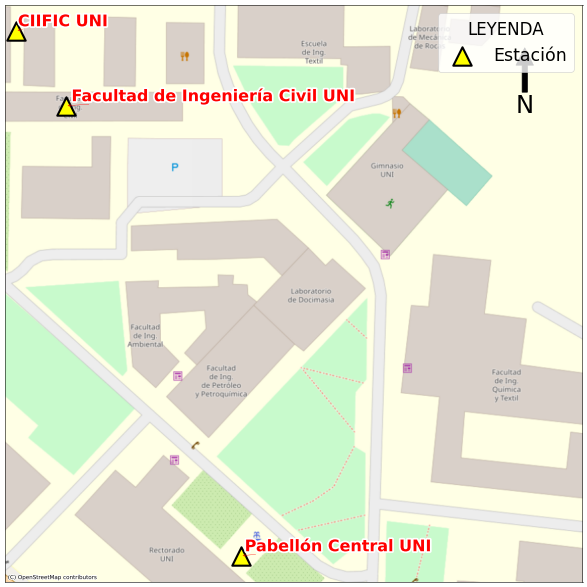
\includegraphics[trim={1mm 1mm 1mm 1mm},clip,width=\textwidth]{Mapa02.png}}
\end{figure}

\vspace{1cm}

\noindent
A continuación, en el \hyperlink{anexoA}{\textbf{Anexo A}} se muestran los registros Tiempo Historia con sus Espectros de Fourier, mientras que
en el \hyperlink{anexoB}{\textbf{Anexo B}} se muestran los Espectros de Respuesta para cada estacion.

\newpage

\clearpage

\vspace*{\fill}% * is needed here
\noindent
\raisebox{0.8cm}{
\makebox[\textwidth]{\hfill {\fontsize{30}{10}\selectfont \hypertarget{anexoA}{ANEXO A}\\ \\ \\ }\hfill }
}
\raisebox{-0.5cm}{
\makebox[\textwidth]{\\ \\ \hfill {\fontsize{24}{20}\selectfont REGISTROS TIEMPO HISTORIA \\  } \hfill }
}
\raisebox{-1.0cm}{
\makebox[\textwidth]{\\ \\ \hfill {\fontsize{24}{20}\selectfont ESPECTROS DE FORURIER \\  } \hfill }
}
\vfill

\clearpage
    
\begin{pycode}
for i in range(event.station.shape[0]):
    channel = event.station.iloc[i]["Channels"]
    fig = event.station.iloc[i]["Graf Acc_Four"]
    for j in range(3):
        capth = 'Registro de Acerelaciones y Espectros de Fourier de la estación %s en dirección %s.' %(event.station["Id"].iloc[i], channel[j])
        print(r'\begin{figure}[!ht]')
        print(r"\caption{%s}"%capth)
        print(r"\label{fig: figura_%s}" %fig[j].split('.')[0])
        print(r"\centering")
        print(r"\includegraphics{%s}"%fig[j].split('.')[0])
        print(r"\end{figure}")
        print(r'\newpage')
print(r"\clearpage")
\end{pycode}
\newpage

\vspace*{\fill}% * is needed here
\noindent
\raisebox{0.8cm}{
\makebox[\textwidth]{\hfill {\fontsize{30}{10}\selectfont \hypertarget{anexoB}{ANEXO B}\\ \\ \\ }\hfill }
}
\raisebox{-0.5cm}{
\makebox[\textwidth]{\\ \\ \hfill {\fontsize{24}{20}\selectfont REGISTROS TIEMPO HISTORIA \\  } \hfill }
}
\raisebox{-1.0cm}{
\makebox[\textwidth]{\\ \\ \hfill {\fontsize{24}{20}\selectfont ESPECTROS DE RESPUESTA \\  } \hfill }
}
\vfill


\clearpage
    
\begin{pycode}
for i in range(event.station.shape[0]):
    fig = event.station.iloc[i]["Graf Acc_Sa"]
    capth = 'Registro de Acerelaciones y Espectros de Respuesta de la estación %s en las 3 direcciones.' %(event.station["Id"].iloc[i])
    print(r'\begin{figure}[!ht]')
    print(r"\caption{%s}"%capth)
    print(r"\label{fig: figura_%s}" %fig.split('.')[0])
    print(r"\centering")
    print(r"\includegraphics{%s}"%fig.split('.')[0])
    print(r"\end{figure}")
    print(r'\newpage')
print(r"\clearpage")
\end{pycode}
\newpage

\listoffigures

\listoftables

\newpage

\end{document}

